\section{Multiple States of the Human Being}

\begin{quotex}
Thou hast ordered all things in measure and number and mass. \flright{\textsc{Wisdom of Solomon 11:20}}

A science was less esteemed for itself than for the degree in which it expressed after its own fashion and represented within a certain order of things a reflection of the higher immutable truth which anything of any reality necessarily partakes of. \flright{\textsc{Rene Guenon}, \textit{East and West} }

\end{quotex}
\paragraph{Namarupa}

\begin{wrapfigure}{rt}{0.35\textwidth}
\centering
 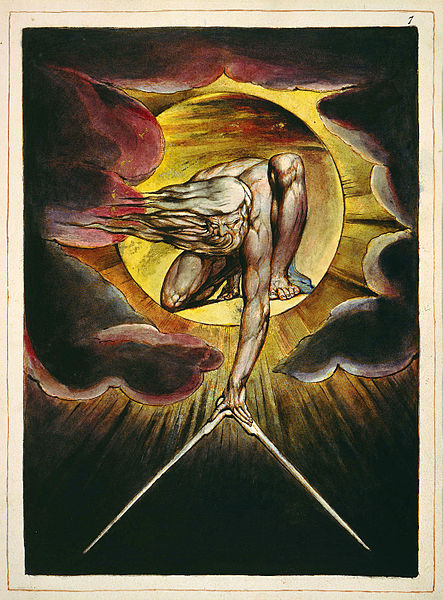
\includegraphics[scale=1]{a20200621MultipleStatesoftheHumanBeing-img001.jpg}
\caption{Ancient of Days}
\end{wrapfigure}

Moving on from Vaisesika to Advaita Vedanta, particularly as explained by \textbf{Adi Shankara}, we will focus on the teachings on the world of nature. Namarupa, literally meaning “name and form” constitute an object or being. They correspond to the intelligible and sensible aspects, or, in different words, “form and matter” or “essence and substance”. This shows why English is a poor language to express metaphysical concepts, since the words are not precise — “form” is used in two different senses.

Nevertheless, this concept is identical to Platonism and Scholasticism, which represent the peak metaphysics of the ancient and medieval Europeans. The point is that our experience includes the senses as well as thought. The experience is incomplete until the mind makes a judgment about what it is. Although the senses and thought are not one, there is no dualism of thought and extension in the Cartesian sense: it is nondual.

Everything that exists, has name and form. Physics, then, is the study of the world of matter, i.e., “becoming”, and Metaphysics, then, is the study of the world of ideas or essences, i.e., “being”. Apart from Adam, who was infused with an intuition of essences (he “named” the animals), we start with the senses and move on from there to an understanding of ideas. Hence, we can accept physics while rejecting the claim that science is the sole and exclusive form of knowing. Rather, properly understood, physics can illustrate metaphysical principles.

It is pointless to denigrate modern science, since the technological consequences of physics are all too evident all around us, for better or worse. Human flourishing cannot depend on the revival of “traditional” sciences like chiromancy (“palm reading”) or astrology. I have had my palm read and my natal chart interpreted — good fun, but limited applicability.

Vladimir Solovyov had a deeper understanding of things, as described in \textit{The development of mind}\footnote{\url{https://www.gornahoor.net/?p=3514}}. Science, philosophy, and theology are three forms of knowing, at increasing depths. Since, as Guenon claimed, time is not neutral, but is qualitative. This means that events occur at time periods that is proper for them, not at random or without sufficient reason. Hence, the notion of development in time a necessary consequence.

\paragraph{Elements}
The elements and their properties in Advaita are basically same as in the Vaisesika system, since both orthodox schools follow the Upanishads. These elements are qualitative and therefore not part of physics. Nevertheless, as was shown in the case of the element fire or light, it does have real world effects. Another example is the element Akasha, or ether, which fills empty space. Einstein famously rejected the existence of the ether since he understood it only in terms of physical matter. However, the Void, i.e., “empty space”, is not a possibility of manifestation. Nature abhors a vacuum. So we should not be surprised when physics find that the so-called vacuum is actually quite busy. See \textit{The Vacuum State}\footnote{\url{https://en.wikipedia.org/wiki/Vacuum_state}}, for example.

\paragraph{Atomism and Continuity}
God has ordered all things by measure, number, and mass. For the first two, we have these relationships:

Measure = geometry = continuous

Number = arithmetic = discrete or atomistic

Measure, as continuous, can be indefinitely divided. On the other hand, atoms are the smallest parts which cannot be further divided. Vaisesika holds the atomistic view whereas Advaita claims the other. Which is correct, since both systems are orthodox? If we turn to physics, we see that both are true. For example,

\begin{enumerate}
\item Light is both a wave – that is, continuous – and a photon, that is, an atom of light 
\item Electrons likewise act like waves or particles, depending on circumstance. 
\end{enumerate}
This can go on. Physics cannot explain this phenomenon, but metaphysics can.

\paragraph{States of Being}
Inorganic nature serves a purpose which lies beyond it; that is because it does not have its own self-organizing principle. The division of inorganic nature if somewhat arbitrary. Where does one mountain begin and another end? What are the precise boundaries of the oceans?

Organic things are likewise composed of the same elements as inorganic nature. In addition, a new principle comes into play: viz., the power of life. Life realizes a state of greater perfection through its power of realising an ideal. Here are examples of states of greater perfection, from lowest to highest.

\begin{itemize}
\item \textbf{Stone}. A stone does not live, since it has no tendency to become perfect, no inward inclination or strength to turn itself into a pillar or a statue.
\item \textbf{Plant}. A plant lives. If placed in suitable conditions, it has the power to grow, put forth leaf and blossom, flower and fruit. 
\item \textbf{Animal}. An animal is capable of a fuller life than the plant. It sees, hears and feels, and also knows vaguely what it is about. Not only does it thrive in favourable conditions, but it goes out to find those conditions. It moves on purpose, while the plant does not. 
\item \textbf{Human}. The human being lives a much higher life. He is a reflective being, with understanding and will. He has the growing power of the plant, the moving and the sensing powers of the animal, as well as the power to pierce behind the veil, discriminate the eternal from the non-eternal, choose between good and evil. 
\item \textbf{Angelic states}. Men who realise their ambition are the gods. 
\item \textbf{Jivanmukta}. The realisation of the Supreme Identity or Beatific Vision. Someone who has achieved self-realisation. 
\end{itemize}
Each state of being is ontologically different from the others. Just working out in the gym does not result in an ontological change, as some wannabe traditionalists have claimed. The human state encompasses all the lower states, but adds the intellectual soul. It should be obvious from the description that biology or evolutionary psychology cannot explain it.

The human state relies on rational thinking, which is sequential and therefore subject to time. When a man has realised his possibilities, he has reached an angelic state (“gods” as Radhakrishnan puts it). In this state, there is a direct understanding through intuition, which is immediate and beyond time. It is more like an “aha” experience than logical demonstration. This is the Edenic state, before the Fall. Thomas Aquinas describes it this way:

\begin{quotex}
In paradise man would have been like an angel in his spirituality of mind, yet with an animal life in his body. 

\end{quotex}
He goes into more detail about angelic states in \textit{Treatise of separate substances}\footnote{\url{https://isidore.co/aquinas/SubstSepar.htm}}.

Even beyond this state, there is the Beatific Vision, achieved by few. Aquinas elaborates on this description of the Beatific Vision or Supreme Identity:

\begin{quotex}
Man was happy in paradise but not with that perfect happiness to which he was destined, which consist in the vision of the Divine Essence. 

\end{quotex}

\paragraph{Appendix}
The study of the metaphysics or the Hindu schools does not mean that we have to accept the mythologies of the Ramayana or Mahabharata, apart from the Bhagavad Gita.

As should be clear, the Medieval and Ancient metaphysics of the West are equivalent to that of the East. Westerners can study Eastern systems either to enrich or recover Western tradition. Those Westerners who fail to recognize this and instead embrace in toto those of the East typically show their misunderstanding of both.

Some unacknowledged quotations are from Indian Philosophy, Volume Two, by \textbf{Sarvepalli Radhakrishnan}.

\flrightit{Posted on 2020-06-21 by Cologero }

\begin{center}* * *\end{center}

\begin{footnotesize}\begin{sffamily}



\texttt{Draft Horse on 2020-06-24 at 03:05 said: }

A good post, but I think you write off the traditional sciences too readily, especially astrology. 

In a “practical” sense, done properly it can identify a persons talents, and show them the most important days/times of their life, along with helping them avoid danger. 

More importantly, it can facilitate in the astrologer (who is suitably disposed) an easier understanding of higher metaphysical principles, particularly the ones written about in Symbolism of the Cross. Then there is also the alchemical usages, hinted at by Evola in his book on the subject. 

Of course astrology today has been co-opted by counter traditional forces, but it still has a capacity for higher use in the right hands, at least that's what I believe anyway. 

So, in short, I think it does have a great value for people today, especially those who are on a spiritual path.

A minor point in your post, but it caught my attention.


\hfill

\texttt{Cologero on 2020-06-28 at 09:54 said: }

I can't dispute your point in an absolute sense. Astrology at least recognizes that the time and place of one's birth is are necessary conditions of life, whereas the modern mind will typically consider them to be arbitrary and even unjust. Moreover, the planets are analogous to the subtle centers in the body. (See Oscar Hinze on Tantra Vidya\footnote{\url{https://www.gornahoor.net/?p=8618}}).

Whether there is benefit in a practical sense depends on the existence and availability of reliable astrologers.


\end{sffamily}\end{footnotesize}
